\chapter{Evaluating and Testing}
Now that we have taught our interactive lessons, we need to be sure our students have actually obtained knowledge.  We can do this through formal and informal evaluations.\\
  
Informal evaluations can usually be done during or at the end of class, to ensure everyone is on the same page.  Examples of informal evaluations would be:

\begin{itemize}
 \item Quizzing students verbally
 \item Competition between boys and girls to answer questions
 \item Using flashcards to test understanding
 \item Doing games or races with students to find the answer
\end{itemize}

Informal evaluation is useful because you can quickly see whether students have understood the information presented and if certain topics need to be taught again.  However, it is more difficult monitoring long-term progress of individual students or pin pointing issues the students may be struggling with.\\

Formal evaluations are homework, tests, and quizzes which would receive a grade.  These grades can be tracked overtime, and used as an indicator of student progress.  However, tests usually come at the end of a topic, and may be too late for a teacher to re-teach the topic if it was found completely misunderstood by students. To best serve our needs, examinations should:

\begin{itemize}
 \item Follow the NECTA format
 \item Find a balance between the difficulty of NECTA exams and what is taught in class
 \item Have some questions from previous NECTA  exams on the test
 \item Test on the material you have provided your students
\end{itemize}

When you get tired of students failing, test their collective knowledge with a group test.  Write one question on the board at a time and select a student at random to answer it.  All students get the collective grade.  May encourage your stronger students to help the ones who don't study.  To avoid cheating, make sure the class is silent and have the student come to the board before you write the question.

We can also evaluate our own work.  We can ask students to evaluate our course through a questionnaire or discussion.  This promotes genuine interaction, develops a much greater awareness among students of what is happening in the classroom, and helps you understand better how they react to your teaching. See the section on Teacher Evaluation later in this chapter.

\section{Test Content}

We hope to teach our students a combination of knowledge and application of the newly learned information.  By using Bloom's cognitive levels, we can evaluate the outcomes of our instruction.

\begin{center}
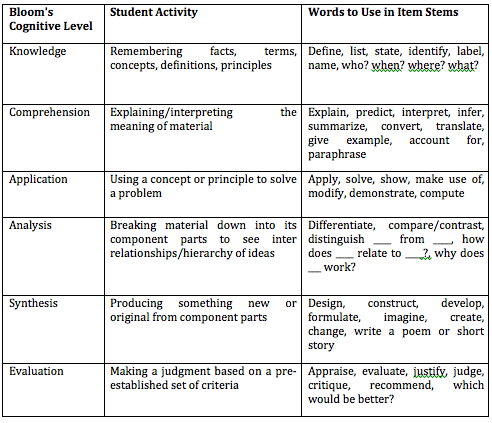
\includegraphics[scale=1]{./img/picture-8.png} 
\end{center}

When writing a test we also want to ensure that the number of questions we include on that test represents the amount of time we spent teaching those concepts in class.  The easiest way to ensure a representative sample of content and cognitive objectives on the test is to prepare a table of specifications. This table lists the content topics on one dimension and the cognitive skills on the other. We want to include content and skills in the same proportion as they were stressed during instruction.\\

\begin{figure}[h!]
\begin{center}
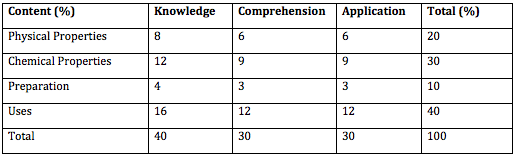
\includegraphics[scale=1]{./img/picture-9.png}
\caption{Table of Specification for a Chemistry Unit Test on Oxygen}
\end{center}
\end{figure}

This table indicates the content topics, the objectives to be covered and the proportion of the test that will be devoted to each. Evidently, more class time was spent on the uses of oxygen because 40\% of the test questions deal with uses compared with only 10\% on preparation. The column totals indicate that 40\% of the items will be written at the knowledge level with the remaining divided equally between comprehension and application. Using the percentages assigned to each cell, we can write the appropriate number of items. For example, because 20\% of the test is to cover physical properties and 30\% is to be application, then 6\% of the total test would measure the ability to apply knowledge about oxygen's physical properties to new situations.\\

Using a table of specifications aligns test content with instruction content, ensuring content validity of the test.  Using a table of specification also helps an instructor avoid one of the most common mistakes in classroom tests, namely writing all the items at the knowledge level.

\section{Format}

As mentioned earlier, we want to ensure that our test format reflects the style of questions that will be on the NECTA exam.  Most NECTA exams contain the following format:

\begin{enumerate}
 \item Form II
 \begin{enumerate}
  \item Multiple Choice, Matching, and True and False
  \item Short Answer
  \item Guided Essay
 \end{enumerate}
 \item Form IV
  \begin{enumerate}
  \item Multiple Choice and Matching
  \item Short Answer
  \item Essay
 \end{enumerate}
\end{enumerate}

Therefore, our examinations should include similar style of questions so that our students are not seeing these types of questions for the first time when they sit for the NECTA exam.   We can prepare questions in advance from previous NECTA exams by creating a question bank, sorted by form and topic.  This helps us in two ways: (1) it shows what topics are most commonly asked on NECTA exams, (2) it allows teachers to quickly find questions from NECTA to use on their tests. 

\section{How to Write a Better Test}

As noted before, assessing and evaluating students learning process is essential for the student and teacher in order to improve.  Therefore, it is important that we create tests that assess our students knowledge properly and encourage them to study. Below are a list of common problems when writing tests:

\begin{enumerate}
 \item Tests include too many questions measuring only knowledge of facts. One of the most common complaints from students is that the test content did not reflect the material discussed in class or what the professor seemed to indicate was most important. This may happen because knowledge questions are the easiest to write.
 \item Too little feedback is provided. If a test is to be a learning experience, students must be provided with prompt feedback about which of their answers were correct and which were incorrect.
 \item The questions are often ambiguous and unclear.  Ambiguous questions often result when instructors put off writing test questions until the last minute. Careful editing and an independent review of the test items can help to minimize this problem.
 \item The tests are too short to provide an adequate sample of the body of content to be covered. Short tests are not fair to students.
 \item The number of exams is insufficient to provide a good sample to students' attainment of the knowledge and skills the course is trying to develop. 
\end{enumerate}

\section{Grading}

Give partial points for correct answers, especially in Mathematics or calculation questions.  Give full points for correct answers, half points for correct procedure, but poor calculations, and no points if no attempt was made.  Write a making scheme that outlines the marks awarded for each question at the time of writing the test.

\begin{figure}[h!]
\begin{center}
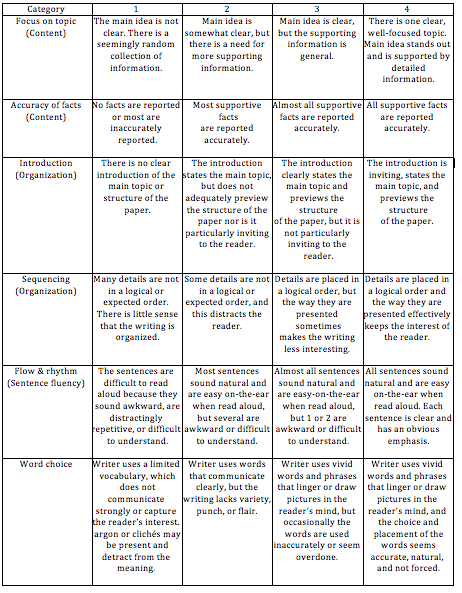
\includegraphics[scale=1]{./img/picture-10.png} 
\caption{Rubric for Grading an Essay}
\end{center}
\end{figure}

When grading essays or other writing, create a rubric.  Give a number of points for organization/format, content, and grammar and spelling.  For example, on a 20 point essay, 5 points are allotted to format, with 1 point being poor and 5 being excellent.  10 points are awarded to content, each point made in the essay 1 point and additional 2 points for explanation of the point.  The 5 remaining points are for grammar and spelling, 1 point for poor and 5 for excellent.


\section{Teacher Evaluation}
Skills of good teaching are developed over many years of teaching. The skills to develop include:
\begin{itemize}
\item Planning and Preparation
\item Classroom Environment
\item Instruction
\item Professional Responsibility
\end{itemize}

\subsection{Importance of Teaching Rubric}
Teaching rubrics have been developed over the years to assist teacher to grow in their teaching.  Self evaluation is one way of developing better teaching skills. Working together will other teachers formally or informally also hones our skills.  The use of a teaching rubric is essential to promote our own growth as a teacher.Below you will find an example of a teacher evaluation.  This guide is used to give meaning to PC evaluation which will be used during your internship teaching evaluations.  

%\subsection{Feedback}
%Feedback is a way of giving help, it is a corrective mechanism for the individual who wants to learn to improve his or her teaching skills. There are rules for giving helpful and construct feedback.
%\begin{enumerate}
%\item Feedback should only be given to those who ask for it. Feedback can be most helpful when:
%\begin{itemize}
%\item It is descriptive of the recipient's behaviour
%\item It is owned by you, not the comments of others
%\item It is specific to your observations
%\item It is relevant to the present situation
%\item It includes examples whenever possible
%\item It is timely for the recipient's development
%\end{itemize}

%\item Ask for feedback only if you are prepared to receive it and learn from it. Feedback is most useful to you if:
%\begin{itemize}
%\item You specify what you want to know
%\item You do not defend yourself or 
%\item You ask for examples if something is not clear
%\item Listen actively with face and body when receiving feedback
%\item Remember the person giving you feedback is trying to help improve your teaching skills
%\end{itemize}
%\end{enumerate} 
\subsection{Lesson Study}
Lesson Study is a method of improving teaching skills used in Tanzania. Lesson Study is a process where teachers work together to improve lesson planning and lesson instruction. 
This is a new incentive of the Ministry of Education. 
Tanzania has adopted this Japanese method of lesson improvement. The teacher presents a lesson that he has prepared and the other teachers evaluate it. After the teachers evaluate it they discuss the lesson to re-plan it based on the activities/hands-on aspects. The lesson is represented.\\
\textbf{Requirements}
\begin{itemize}
\item{More than one teacher of the subject}
\item{You need teachers to work together}
\end{itemize}
This is a goal of the Ministry that is being implemented as part of in-service training.

\section{Test Taking Skills for Your Students}
The following are suggestions for your students on how to pass their examinations.
\begin{description}
\item[Prepare before the test] By underlining in their exercise book, summarizing notes, and using study groups, students can improve their preparation for a test. Students should also get a good nights sleep at least two nights before the exam.  We are most affected by our sleep cycle 48 hours before, not 24.
\item[Performance during the test] When taking the test, students should follow all directions, answer easy questions first, and watch the time. Students should also give preference to questions that have higher marks, like essay questions. 
\item[Analysis after the test] Students should examine what questions they missed and why.  How can they improve from these mistakes for the next exam.
\item[True and False Questions] Students should assume all questions are true unless they can clearly determine it is false. Remember, all parts of the statement must be true for the statement to be true. Students should also beware of absolutes like all, none, always, never, etc. 
\item[Multiple Choice Questions] Students should always use the process of elimination to reduce the choices. If two answers are synonyms, students should eliminate both of them. If two answers are close in meaning, one of them is usually the correct answer.
\item[Essay] The NECTA format for essays requires students to write an introduction with a definition, five clear points that include definitions, and a conclusion. Students should always attempt to answer essay questions as they are 20 points of the exam or more.
\end{description}

